\documentclass[]{article}
\usepackage{graphicx}

%opening
\title{Introduction to Machine Learning Final Project}
\author{Paula Campaña Donoso $-$ 730723162 \\ Brad Weyand $-$ 730318989 \\ Siwei Han $-$ 730723179 \\ Thomas Kung $-$ 730620459}

\begin{document}

\maketitle

\begin{abstract}
For this project, the idea is to guess between poisonous and non-poisonous mushrooms using binary classification as well as random forests. The dataset that was chosen provides numerous categories for the different aspects of each type of mushroom. There is around 23 species of mushrooms inside this data set, and 23 categories in which this mushorooms are being classified. The first 22 categories help distinguish the characteristics of each of the mushrooms, while the last category determines whether or not the mushroom can be considered poisonous or not. There is a prepocessing section to change the data from strings to integers, then a visualization of the data. After that, the model is being trained and finally the accuracy of the model is being tested in order to see the results from this analysis.
\end{abstract}

\section{Pre-Processing Data}

\subsection{What was it done?}
In order to use the data set for the analysis to guess whether or not the mushrooms are poisounous, the data set needed to be pre-processed to change all the categorical classifications that were registered as strings, into integers. For that reason we started by investigating which could be the best approach to transform the information in order to have a better result for the random forest model. After some research, it was determined that we would have to change the values using One-Hot encoding process. This process would allow us ot have all the classifications in binary outputs $(0,1)$. With this new classification form, we can be able to interpret the data better as there would not be factors such as ranking that interfere in our guessing of the poisonous level of each of the mushrooms, and also it is a form of data interpretation that allows the random forests analyze the data easily and better.

\section{Visualization}
The following image contains different set of graphs that show each category.

\begin{figure}[!htb]
	\centering
	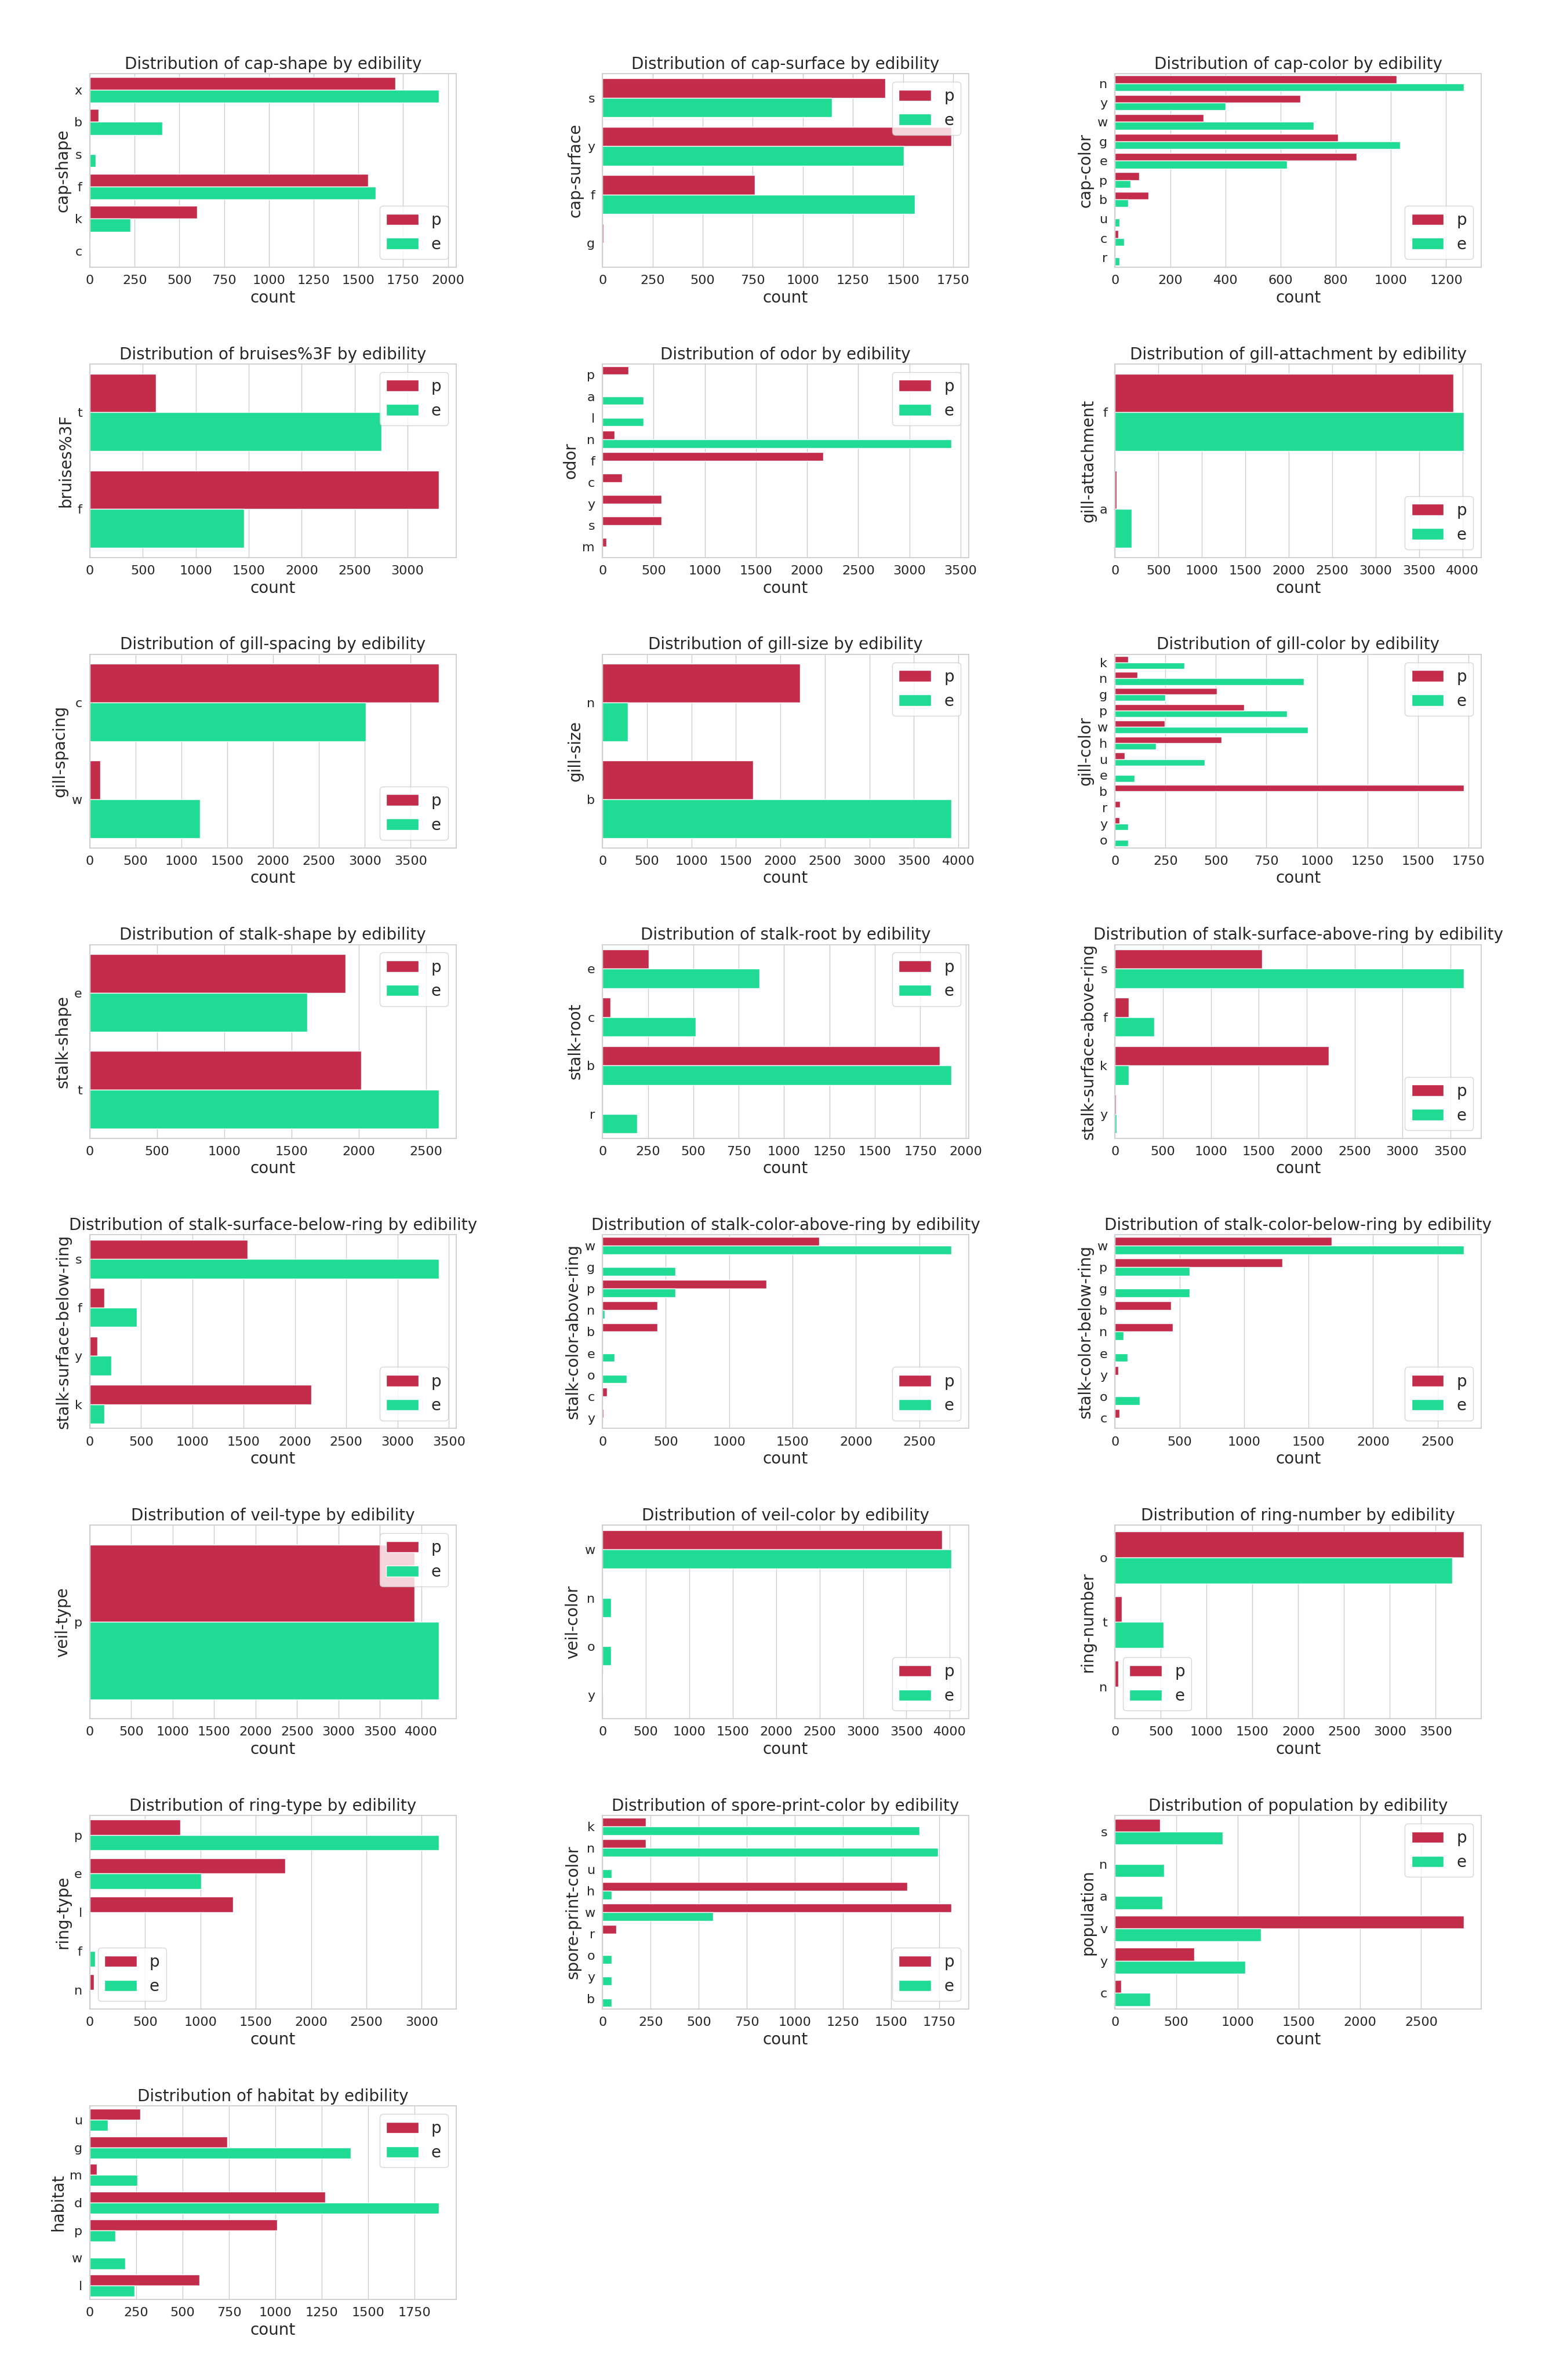
\includegraphics[scale=0.116]{visualize.jpeg}
	\caption{Visualization of data of all categories}
	\label{fig}
\end{figure}


\section{Training Model}

\section{Accuracy of Model}

\end{document}
